\documentclass[../main.tex]{subfiles}
\DoIfAndOnlyIfStandAlone{%
    \externaldocument{linear-block-codes}%
    \setcounter{chapter}{3}%
}%

\begin{document}

    \chapter{Visualisation}

    We consider two kinds of errors: random errors, which are distributed randomly among individual bits; and burst errors, which occur in consecutive groups of hundreds of bits. Burst errors are usually the result of, for example, fingerprints, dust and scratches on the disc surface \autocite{wicker1999reed}.


    Additionally to the BSC as described in \Cref{sec:maximum-likelihood-decoding} we should mention the Binary Erasure Channel (BEC), in case a codeword is transmitted, but nothing is received \autocite{mackay2003information}. Let $c$ be the transmitted code with alphabet $\{0,1\}$, let $r$ be the received code with alphabet $\{0,1,e\}$ where $e$ denotes the erasure. This channel is characterised by the following conditional probabilities:

    \begin{align*}
        P(r=0 | c=0) &= 1-p\\
        P(r=e | c=0) &= p\\
        P(r=1 | c=0) &= 0\\
        P(r=0 | c=1) &= 0\\
        P(r=e | c=1) &= p\\
        P(r=1 | c=1) &= 1-p
    \end{align*}

    \begin{figure}[htp]
        \begin{center}
            \begin{tikzpicture}[
                            > = latex,
                node distance = 4em and 15em,
                   bit/.style = {rectangle, draw=black, thick, minimum size=7mm}
                ]
                % nodes
                \node[bit]    (topleft)                                                 {0};
                \node[bit]    (topright)      [right=of topleft]                        {0};
                \node[bit]    (bottomleft)    [below=of topleft]                        {1};
                \node[bit]    (bottomright)   [right=of bottomleft]                     {1};
                \node[bit]    (erasure)       at \findmid{0.5}{topright}{bottomright}   {$e$};

                % labels
                \node[left=1cm]  at \findmid{0.5}{topleft}{bottomleft}   {$c$};
                \node[right=1cm] at \findmid{0.5}{topright}{bottomright} {$r$};


                % lines
                \draw[->,line width=1pt] (topleft.east) -- (topright.west) node[midway, above] {$1-p$};
                \draw[->,line width=1pt] (topleft.east) -- (erasure) node[pos=0.9, above] {$p$};

                \draw[->,line width=1pt] (bottomleft.east) -- (bottomright.west) node[midway, below] {$1-p$};
                \draw[->,line width=1pt] (bottomleft.east) -- (erasure)  node[pos=0.9, below] {$p$};
            \end{tikzpicture}
        \end{center}
        \caption{Model of the binary erasure channel (BEC)}
        \label{fig:binary_erasure_channel}
    \end{figure}

    Cross-interleaved Reed-Solomon code (CIRC) is well suited to deal with combinations of random as well as burst errors. For example, CIRC is used in compact discs with requirements such as:

    \begin{itemize}
        \item low redundancy;
        \item the ability to correct random errors and burst errors;
        \item good possibility of error concealment in case the correction capacity is surpassed.
    \end{itemize}


    \section{Bit Stream Encoding}
    An analog-to-digital converter (ADC) converts sound into a digital data stream at a sample rate of 44.1 kHz, which, according to Nyquist's sampling theorem, is sufficient to reproduce a maximum audio frequency of 20 kHz. The 32-bit stereo sample has 16 bits for the left and 16 bits for the right channel. Six of these samples are then grouped in a frame of 32 audio bits, 16-bit per audio channel. The net audio bit stream is therefore $44100 \times 32=1.41 Mbits/s$. These samples are then each divided to form 24 8-bit symbols per frame. \Cref{fig:bit_streams} shows this as bit stream $B_1$. In $B_2$, 8 parity symbols and a control and display symbol (C \& D) are added such that each frame now contains 33 data symbols. The C \& D symbol contains information for the listener which can be shown if the player has a display. Subsequently an eight-to-fourteen (EFM) code is used to translate these into 14-bit symbols plus three merging bits in $B_3$. This brings the net data bit stream rate to $1.94 Mbits/s$. Then a synchronisation pattern of 27 bits is added to the frame to obtain bit stream Bi of $33 \times 17+27=588$ channel bits per frame in such a way that each 1 indicates a pit edge; it therefore makes no difference if pit and land were interchanged on a disc. The total bit rate after all these data manipulations is approximately $4.32 Mbits/s$ \autocite{wicker1999reed}.

    \newpage

    % Test page for figures
    %----------------------------------------------

    \begin{figure}[h!tp]
        \centering
        \begin{bytefield}{32}
            \begin{rightwordgroup}{\scriptsize 1 frame}
                \wordbox{1}{}
            \end{rightwordgroup} \\
            \begin{rightwordgroup}{\scriptsize 32 bits per sampling period}
                \bitbox{8}{1011001}
                \bitbox{8}{01110010}
                \bitbox{8}{1000111}
                \bitbox{8}{01010010}
            \end{rightwordgroup} \\
            \begin{rightwordgroup}{\scriptsize 4 symbols of 8 bits}
                \bitbox{8}{8 bits}
                \bitbox{8}{8 more bits}
                \bitbox{8}{8 more bits}
                \bitbox{8}{8 more bits}
            \end{rightwordgroup} \\
            \wordbox{2}{A 32-bit field. Note that text wraps within the box.}\\
            \bitbox{1}{1}  \bitbox{1}{0}  \bitbox{1}{1}  \bitbox{1}{1}
            \bitbox{1}{1}  \bitbox{1}{0}  \bitbox{1}{0}  \bitbox{1}{1}
        \end{bytefield}
    \end{figure}

    %----------------------------------------------

    \begin{figure}[h!tp]
        \centering
        \begin{tikzpicture}[
                        > = latex,
               bit/.style = {rectangle, draw=black, thin, minimum size=2.5mm},
            sample/.style = {rectangle, draw=black, thin, minimum size=2.5mm, inner xsep=1em, outer xsep=0pt},
            symbol/.style = {},
              grey/.style = {fill=gray!25},
            wordbox/.code = {\\\wordbox{1}{Field: #1}},
             bitbox/.code = {\\\bitbox{1}{#1}},
            ]
            \node {
                \begin{bytefield}{8}
                    \wordbox{1}{Source: A}
                    \tikzset{wordbox/.list={1,2,3}}
 %                   \tikzset{bitbox/.list={0,1,2,3,4,5,6,7}}
                \end{bytefield}
            };
        \end{tikzpicture}
    \end{figure}

    %----------------------------------------------

    \begin{figure}[h!tp]
        \centering
        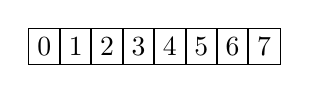
\begin{tikzpicture}[
                        > = latex,
               bit/.style = {rectangle, draw=black, thin, minimum size=2.5mm},
            sample/.style = {rectangle,
                            draw=black,
                            thin,
                            minimum size=2.5mm,
                            inner sep=0pt,
                            outer sep=0pt},
            symbol/.style = {},
              grey/.style = {fill=gray!25},
            wordbox/.code = {\\\wordbox{1}{Field: #1}},
             bitbox/.code = {\\\bitbox{1}{#1}},
            ]

            \foreach \x in {0,...,7}{%
                \node[bit] at (\x/2.51,0) {$\x$};
            }
        \end{tikzpicture}
    \end{figure}

    %----------------------------------------------

    \begin{figure}[h!tp]
        \centering
        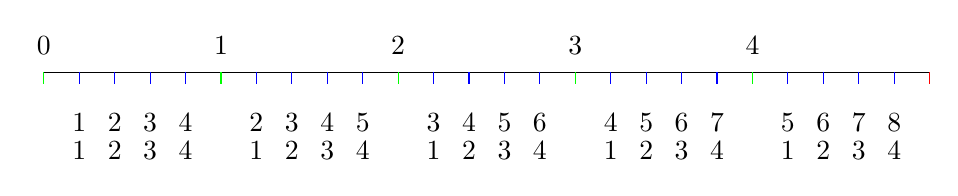
\begin{tikzpicture}[scale=0.75]
            \draw (0,10)-- (15,10);
            \foreach \x in {0,...,4}{
                \draw[draw=green] (3*\x,10)--++(0,-0.2) node[above=2.5mm]{\x};
                \foreach \y [evaluate=\y as \j using int(\x+\y)]in {1,...,4}
                    \draw[draw=blue] ({3*(\x+\y/5)},10)--++(0,-0.2)
                    node[below=2.5mm]{\j}
                    node[below=6mm]{\y};
            }
            \draw[draw=red] (3*5,10)--++(0,-0.2);
        \end{tikzpicture}
    \end{figure}

    %----------------------------------------------

    \newpage

    %----------------------------------------------

    \newcommand{\bits}[4]{
        \begin{bytefield}[
                bitformatting={\tiny\bfseries},
                bitwidth=auto,
                bitheight=9pt,
                bitwidth=0.01\linewidth
            ]{32}
            \bitbox{8}{\tiny$#1$}
            \bitbox{8}{\tiny$#2$}
            \bitbox{8}{\tiny$#3$}
            \bitbox{8}{\tiny$#4$}
        \end{bytefield}%
    }%

    \newcommand{\periods}[1]{
        \begin{bytefield}[
                bitformatting={\tiny\bfseries},
                bitwidth=auto,
                bitheight=9pt,
                bitwidth=0.01\linewidth
            ]{#1*8}
%            \begin{rightwordgroup}{\scriptsize1 frame}
                \wordbox{1}{frame}\\
%            \end{rightwordgroup} \\
%            \begin{rightwordgroup}{\scriptsize6 sampling periods}
            \foreach \x in {1,...,#1} {%
                \bitbox{8}{\tiny\x}
            }
%            \end{rightwordgroup} \\
        \end{bytefield}%
    }%

    \begin{figure}[h!tp]
        \centering
        \begin{tikzpicture}[
                        > = latex,
               bit/.style = {rectangle, draw=black, thin, minimum size=2.5mm},
            sample/.style = {minimum size=2.5mm,
                            inner sep=0pt,
                            outer sep=0pt},
            symbol/.style = {align=center, inner sep=0pt, fill=gray!15},
             frame/.style = {fill=gray!25, circle, draw=blue},
            wordbox/.code = {\\\wordbox{1}{Field: #1}},
             bitbox/.code = {\\\bitbox{1}{#1}},
            ]
            % 1 frame
            \coordinate (frame) at (0,0);
%            \coordinate (time) at (4,0.5);
%            \draw[<->] (frame) -- +(6cm,0);
%            \draw[->] (time) -- +(1cm,0) node[right]{t};

            % 6 sampling periods
            \node(samples)
                [sample,below=of frame]
                {\periods{6}};

            % 32 bits per sampling period
            \node(period)
                [symbol, below=of samples.south west, label=right:{\tiny32 bits per sampling period}] {\bits{10111001}{01110010}{10001111}{01010010}};

            % 4 symbols of 8 bits
            \node(symbols)
                [symbol, below=3mm of period,  label=right:{\tiny4 symbols of 8 bits}]
                {\bits{ }{ }{ }{ }};

            % 24 audio symbols


            % connecting symbols
            \draw[dotted] (period.south west) -- (symbols.north west);
            \draw[dotted] \findmid{0.5}{period.south west}{period.south} --
                          \findmid{0.5}{symbols.north west}{symbols.north} ;
            \draw[dotted] (period.south) -- (symbols.north);
            \draw[dotted] \findmid{0.5}{period.south east}{period.south} --
                          \findmid{0.5}{symbols.north east}{symbols.north} ;
            \draw[dotted] (period.south east) -- (symbols.north east);

            % connecting periods to one sampling period
            \draw[dashed] \findmid{0.333}{samples.south west} {samples.south} -- (period.north west);
            \draw[dashed] \findmid{0.667}{samples.south west} {samples.south} -- (period.north east);



        \end{tikzpicture}
        \caption{Bit streams in the encoding process}
        \label{fig:bit_streams}
    \end{figure}

    %----------------------------------------------


    \section{Cross-interleaved Reed-Solomon Code}


    \section{Decoding}

\end{document}
